\documentclass{article}%
\usepackage[T1]{fontenc}%
\usepackage[utf8]{inputenc}%
\usepackage{lmodern}%
\usepackage{textcomp}%
\usepackage{lastpage}%
\usepackage{authblk}%
\usepackage{graphicx}%
%
\title{FOXO4{-}Knockdown Suppresses Oxidative Stress{-}Induced Apoptosis of Early Pro{-}Angiogenic Cells and Augments Their Neovascularization Capacities in Ischemic Limbs}%
\author{Cindy Rivera}%
\affil{Neurophysiology Laboratory, Department of Pharmacology and Experimental Neuroscience, University of Nebraska Medical Center, Omaha, Nebraska, United States of America}%
\date{01{-}01{-}2013}%
%
\begin{document}%
\normalsize%
\maketitle%
\section{Abstract}%
\label{sec:Abstract}%
Immune cells may be able to generate undesirable body reactions in order to fight infectious diseases, according to a new study by UCSF scientists. This finding provides direct evidence of the cells determination of common cellular molecular mechanisms, including the process for introducing new cells into the body.\newline%
The study, published online Dec. 22, 2012, in Cell, details the molecular mechanism under which cells produce the sweet chemical fatty acids known as adipose glycosides that form adipocytes, a group of cells that build bone, skin and cartilage.\newline%
Study Results\newline%
The findings further point to the role of the laser touch principle in the body and the importance of the genes that produce adipocytes. As a result, the findings may be applied to fight infectious diseases, such as HIV.\newline%
According to the researchers, Our findings suggest that Adenominas, a group of about 100 pre{-}laser{-}like nerve cells, are able to turn other adipocytes into precursor cells that produce forms of fatty acids that can reduce appetite. If the regulatory pathway can be identified, an enteropathogenic pathway or metabolic pathway may be designed to inhibit the production of adipocytes for human and mouse studies.\newline%
Drug as Potential Therapeutic Product\newline%
Cells are efficient at the motions that enable cellular functions, such as proliferation, differentiation and differentiation into adipocytes. In particular, the adipocyte cells can produce NAD, a compound that is essential for building fat and for increasing an organisms appetite and energy levels.\newline%
Recently, scientists found that adipocytes do this for themselvesnot to produce N but to create quantities of a particular type of fat. This discovery led the researchers to contemplate ways to increase the production of other types of fatlike those that produce lipids or promote blood clotting.\newline%
Contact: Anna Grasselli, University of California San Francisco, r.grasselli@ucsf.edu, (415) 274{-}2470

%
\subsection{Image Analysis}%
\label{subsec:ImageAnalysis}%


\begin{figure}[h!]%
\centering%
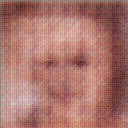
\includegraphics[width=150px]{500_fake_images/samples_5_481.png}%
\caption{A Close Up Of A Person Wearing A Tie}%
\end{figure}

%
\end{document}